%% Classe de documento e opções
\documentclass[%% Opções: [*] comente para remover; [>] passada para pacotes
  article,%% Tipo de documento: article, book, report, etc. [>]
  a4paper,%% Tamanho de papel: a4paper, letterpaper, etc. [>]
  12pt,%% Tamanho de fonte: 10pt, 11pt, 12pt, etc. [>]
  fleqn,%% Alinhamento de equações à esquerda (comente para centralizado) [>]
  oneside,%% Impressão: oneside (anverso) ou twoside (anverso e verso) [>]
  % twocolumn,%% Texto em duas colunas (comente para uma coluna) [>]
  chapter = TITLE,%% Títulos de capítulos em maiúsculas [*]
  section = TITLE,%% Títulos de seções (secundárias) em maiúsculas [*]
]{abntex2}

%% Pacotes utilizados
\usepackage[%% Opções
  BibURLs = false,%% Links de URLs nas referências: true ou false
  ABNTNum = none,%% Estilo numérico ABNT: none (AUTOR, ANO), dflt (1) e brkt [1]
]{unoesc-article}

\usepackage{caption}




%% Arquivo de referências
\addbibresource{unoesc-article.bib}

%% Informações do documento
%%%% Título
\titulo{AUTOMAÇÃO DE HORTAS RESIDENCIAIS URBANAS: estudo de caso em uma residência}
%%%% Título em outro idioma
% \titleinenglish{%
%   Title of the academic work or%
%   \nextline scientific article or research project%
% }
%%%% Autor(es) e afiliação(ões)
\autor{%
  Samuel Ferreira da silva%
  \thanks{%
    \affil{Bacharel Sistemas de Informação; UNOESC ; Chapecó}%
    \sep\email{samuel.silva@unoesc.edu.br}%
  }%
  \and Prof. Jacson Luiz Matte%
  \thanks{%
    \affil{Especialista em Desenvolvimento de aplicações Web; UNOPAR; Chapecó}%
    \sep\email{jacson.matte@unoesc.edu.br.}%
  }%
  % \and Terceiro(a)~M.~Autor(a)%
  % \thanks{%
  %   \affil{Formação, Entidade, Cidade}%
  %   \sep\email{autor3@dominio}%
  % }%
  % \and Quarto(a)~M.~Autor(a)%
  % \thanks{%
  %   \affil{Formação, Entidade, Cidade}%
  %   \sep\email{autor4@dominio}%
  % }%
  % \and Quinto(a)~M.~Autor(a)%
  % \thanks{%
  %   \affil{Formação, Entidade, Cidade}%
  %   \sep\email{autor5@dominio}%
  % }%
}

\data{}

%% Ferramenta para criação de índices
\makeindex%
\crefname{figure}{Figura}{Figuras}
\crefname{table}{Quadro}{Quadros}
%% Início do documento
\begin{document}

\pretextual%% Elementos pré-textuais

\begin{paginadetitulo}%% Página de título

    \begin{ambienteresumo}%% Resumo
A horticultura é uma atividade muito presente no Brasil e tem atualmente se tornado uma prática muito comum em propriedades urbanas e residenciais. No entanto, esse modelo de agricultura sustentável torna-se inviável por questões de desperdícios e dos custos elevados para implementar um sistema automatizado. Nesse contexto, este estudo apresenta o desenvolvimento de um sistema embarcado para a automação da irrigação de uma horta residencial urbana, utilizando o microcontrolador ESP32 e seu sistema operacional FreeRTOS. O problema abordado é o gerenciamento não adequado da irrigação manual, bem como os desperdícios ou falta de recursos hídricos para as plantas da horta, dificultando o cultivo sustentável. O propósito do trabalho foi criar um protótipo de baixo custo que otimizasse o processo de irrigação, melhorando assim a produtividade e o gerenciamento da horta. A metodologia envolveu a utilização de sensores para medir umidade do solo, temperatura e umidade ambiente, chuva e previsão do tempo, com os dados sendo processados pelo ESP32 para acionar a irrigação conforme necessário. Para fins ecológicos, uma cisterna é integrada para captar e armazenar água da chuva, aumentando a eficiência hídrica. Para um melhor gerenciamento e visualização, foi disponibilizado um dashboard para o usuário acompanhar a automação. Quanto à pesquisa, foi utilizada uma abordagem qualitativa, avaliando os resultados da aplicação da automação e a viabilidade da implementação do protótipo. Os resultados apresentaram uma melhoria significativa, com um percentual acima de 90\% de satisfação. Verificou-se também que a automação de hortas urbanas com tecnologias acessíveis pode viabilizar a produção de alimentos em áreas urbanas de forma sustentável, conservando recursos hídricos e energéticos, e apresentando-se como uma solução de baixo custo para a agricultura urbana.
    \palavraschave{Automação. FreeRTOS. Hortas Residenciais Urbanas. Irrigação. Agricultura Familiar}%% Palavras-chave
    \end{ambienteresumo}
    
    % \begin{ambienteresumo}[Abstract]%% Abstract
    % \begin{otherlanguage*}{english}%% Idioma do abstract
    % The abstract text should place the work in the general context and the importance of the topic studied, briefly describe the objectives, the methodology adopted, the results obtained and the main conclusions, reporting the own contribution, in no more than 250 words.
    % It should contain neither mathematical formulas nor deductions nor bibliographical citations.
    % \palavraschave[Keywords]{word 1.\ word 2.\ word 3\ldots\ (maximum 5).}%% Keywords
    % \end{otherlanguage*}
    % \end{ambienteresumo}

\end{paginadetitulo}

\textual%% Elementos textuais
\newpage
\section{Introdução}\label{sec:intro}

Hortas urbanas representam uma alternativa promissora diante das mudanças radicais de urbanização e do rápido crescimento populacional, oferecendo soluções sustentáveis e inovadoras para os desafios ambientais atuais. Estas hortas promovem o bem-estar e moldam o futuro das cidades ao reintroduzir a interação entre o rural e o urbano, incentivando a agricultura urbana. A crescente preocupação com as mudanças climáticas fomenta a valorização do rural nas áreas urbanas, manifestada em mercados agrários, disponibilidade de alimentos locais, sazonais e orgânicos, e hortas comunitárias. 

Nesse contexto, a Empresa Brasileira de Pesquisa Agropecuária (EMBRAPA) tem sido crucial, oferecendo recursos e parcerias através do projeto Embrapa Hortaliças, para promover a inovação em hortas urbanas. Com foco em garantir uma alimentação de qualidade e sustentável, a EMBRAPA apoia iniciativas que valorizam o cultivo orgânico e utilizam tecnologias acessíveis e de baixo custo, como a automação de hortas e estufas, revolucionando e tornando esses sistemas mais eficientes.

A automação nessas estruturas abrange diversos aspectos, como o controle de temperatura, umidade, iluminação e irrigação automatizada. Sensores avançados monitoram constantemente as condições ambientais, permitindo ajustes remotos para otimizar a produtividade. Além disso, a tecnologia de cultivo vertical tem se mostrado especialmente valiosa em áreas urbanas, permitindo o crescimento de mais plantas em menos espaço.

 Essa abordagem promove a maximização da produtividade e a otimização dos recursos, contribuindo para a sustentabilidade e resiliência das hortas urbanas em meio aos desafios do ambiente urbano contemporâneo. No entanto, o controle sobre a irrigação das hortas urbanas na sua maioria é realizado manualmente, este processo, por sua vez, está sujeito a muitas falhas. Outro ponto importante é que o gerenciamento não adequado da horta acarreta uso excessivo de recursos hídricos, estes por sua vez tornando inviável o cultivo, fazendo com que os produtores abandonem a prática do cultivo residencial e busquem a consumir produtos comercializados.  
 
 A partir do exposto, foi objetivo deste trabalho o desenvolvimento de um sistema embarcado, um protótipo de baixo custo para automatizar uma horta  residencial urbana, visando uma maior produtividade e redução de desperdícios hídricos. Esta pesquisa caracteriza-se de natureza aplicada e abordagem qualitativa, na qual visa atingir os objetivos de forma descritiva e exploratória, por meio de procedimentos de pesquisa bibliográfica e estudo de caso.


\section{REVISÃO BIBLIOGRÁFICA}\label{ssec:teor}

A agricultura de precisão envolve o uso de tecnologias modernas para reduzir perdas localizadas e aumentar a produção agrícola. No entanto, os sistemas de automação são muito importantes nesse contexto por permitirem o controle simultâneo de um número muito maior de fatores do que é possível manualmente \cite{coelho2009agricultura}.

Atualmente, produzir seu próprio alimento em pequenas hortas e pomares voltou a ser uma atividade importante, tanto do ponto de vista nutricional e alimentar quanto do da qualidade de vida, por ser uma atividade física e lúdica. Aquele que cultiva seus próprios alimentos adequadamente não precisa preocupar-se com assuntos complexos, como contaminação microbiológica ou por agrotóxicos, rastreabilidade e consumo de alimentos originados de plantas transgênicas, entre outros, porque tem em suas próprias mãos a opção e a responsabilidade de produzir as hortaliças de forma saudável e isenta de resíduos.

De acordo com \citet{HenzAlcantara2009v2}, uma horta é definida como o local onde se cultivam hortaliças e outras plantas, como ervas condimentares e aromáticas. Tradicionalmente, hortas são estabelecidas em quintais e terrenos próximos a residências e cidades, podendo também ser instaladas em terrenos maiores ou em recipientes menores, como vasos e caixotes. Especificamente, hortas urbanas estão situadas em cidades, bairros, vilas ou em áreas periurbanas.

O termo “horta” origina-se do latim “hortus”, que significa uma propriedade cercada, como um horto ou jardim. As hortas variam em tipos, incluindo hortas comerciais, domésticas, institucionais, escolares e comunitárias, podendo seguir sistemas de produção convencional ou orgânica, ou ainda serem autossustentáveis. A escolha do tipo de horta depende do tamanho, da quantidade de hortaliças cultivadas e do objetivo, que pode variar desde a exploração comercial até o consumo doméstico \cite{HenzAlcantara2009v2}.

\subsection{IRRIGAÇÃO}
A irrigação é uma técnica milenar cuja finalidade é disponibilizar água às plantas para que estas possam produzir adequadamente. A técnica, ao longo dos séculos, vem sendo aprimorada, chegando agora a sistemas pontuais, onde a água é gotejada no momento, local e quantidade correta ao desenvolvimento das plantas. Os diversos sistemas de irrigação disponíveis atualmente no mercado dão aos produtores uma moderna tecnologia de produção agrícola que, juntamente com manejo equilibrado da adubação e tratos culturais, reúnem todas as condições para as plantas poderem expressar todo o seu potencial genético de produção. Entretanto, a escolha do sistema de irrigação deve basear-se em análise técnico-econômica, considerando o tipo de solo, topografia, clima, cultura, custo do equipamento e energia, qualidade de água disponível e mão-de-obra.

Quando se trabalha com agricultura irrigada é importante estabelecer o momento certo de iniciar as irrigações e quanto de água aplicar a uma cultura. Estes são os princípios básicos do manejo “racional” da irrigação. Do mesmo modo, o conhecimento de solos, fisiologia da cultura, períodos críticos de consumo de água e seus reflexos na produtividade são essenciais para o bom manejo de aplicação de água. \cite{Embrapa2008v2}.

\subsubsection{Tipos de Irrigação }	
Conforme a \citet{Embrapa2008v2}, irrigação total aplica toda a água necessária para atender a demanda hídrica da cultura. É o tipo de irrigação mais eficiente, mas também o mais caro. Irrigação suplementar aplica parte da água necessária para atender a demanda hídrica da cultura, sendo complementada pela precipitação efetiva. É o tipo de irrigação mais econômico, mas também o menos eficiente. Irrigação com déficit, aplica apenas uma fração da demanda hídrica da cultura. É o tipo de irrigação que pode ser utilizado em áreas com escassez de água, mas pode prejudicar o desenvolvimento da planta. Irrigação de salvação aplica água em um período curto, geralmente durante uma seca, para evitar perdas de produtividade causadas pela falta de água.

A irrigação por superfície é o método mais antigo e o mais utilizado em todo o mundo. De acordo com \citet{Cuenca1989v2}, a história da irrigação começa com a aplicação de água ao solo utilizando-se a sua superfície para o escoamento por gravidade.
Um dos principais problemas da irrigação por superfície é a baixa eficiência de aplicação, traduzida nos valores de perdas de água por escoamento superficial e percolação, na maioria das vezes superior a 40\%.

Os sistemas de irrigação por aspersão \cref{fig:irigaspersao}, são os mais utilizados nos cultivos, e é atualmente o sistema que melhor se adapta às diferentes condições de produção, tais como: tipo de solo, topografia, características agronômicas e aspectos econômicos. O método de irrigação por aspersão visa imitar a precipitação de chuva sobre as plantações. Nele, um jato de água é emitido pelo aspersor, que se desloca de maneira a abranger a área desejada, executando o processo mecânico de simular a chuva. Estes aspersores desempenham o papel de dispersar água no ar, e com o auxílio da pressão atmosférica, transformam-na em pequenas gotículas que se depositam sobre as plantações e o solo \cite{bernardo2006manual}.

\begin{figure}[!htb]
    
    \begin{minipage}{0.9\textwidth}
        \raggedright\caption{Irrigação por aspersão}
        \label{fig:irigaspersao}
    \end{minipage}%
    
    \begin{minipage}{0.9\textwidth}
        \raggedright
        \includegraphics[width=\linewidth]{Figuras/irrigacao-por-aspersao.jpg}
        \fonte{Imagens da internet}
    \end{minipage}
\end{figure}

Já na irrigação subterrânea, água é aplicada auxílio de mangueiras enterradas no solo dentro do espaço e volume explorado pelas raízes das plantas \cite{bernardo2006manual}.

\subsection{AUTOMAÇÃO DE HORTAS URBANAS }

Automação se dá pela utilização de sistemas lógicos programáveis capazes de funcionar   sem a   intervenção   humana   habitual.  Isto   é, usa-se   uma   gama de equipamentos eletroeletrônicos, sendo   alguns:   controlador   lógico   programável (CLP), atuadores, sensores, indutores, bobinas, visando programar o sistema desejado para que, posteriormente, este funcione de maneira autônoma, eficiente e mais precisa que a intervenção humana \cite{Ribeiro}.

Atualmente o uso de técnicas de instrumentação e automação nos sistemas agrícolas tem auxiliado no manejo das irrigações, indicando a quantidade adequada de água aplicada no solo prevenindo o estresse hídrico das culturas que podem afetar tanto em quantidade, como em qualidade na produção da cultura. No entanto, a quantidade de água requerida e o momento de aplicação dessa água dependem de alguns parâmetros \cref{tab:variaveis_ambientais}, bem como: condições climáticas do local, tipo de cultura, seu estágio de crescimento, profundidade efetiva do sistema radicular e umidade do solo. Sempre que a água proveniente da chuva não for suficiente para atender a demanda hídrica das plantas e a disponibilidade de água do solo for esgotada a níveis que irão provocar redução significativa de produtividade, haverá necessidade de suprir a necessidade hídrica das culturas com a aplicação de água de irrigação \cite{Roque2008}.
 
 Com a utilização da automação, controladores desenvolvidos podem ativar ou desativar sistemas de irrigação com base nos dados enviados continuamente por estes sensores. Um sistema de irrigação automatizado, quando bem programado e calibrado, assegura a umidade ideal para as culturas em cada estágio de desenvolvimento, prevenindo tanto a escassez quanto o excesso de água.\cite{coelho2003desenvolvimento}.

\begin{table}[!htb]
\renewcommand{\tablename}{Quadro}
\captionsetup{justification=raggedright,singlelinecheck=false}
    \caption{Variáveis ambientais importantes para culturas de hortaliças}
    \centering
    \begin{tabular}{| m{4cm} | m{10cm} |}
        \hline
        \textbf{Variável Ambiental} & \textbf{Importância para Culturas de Hortaliças} \\
        \hline
        Temperatura do Ar & Influencia o crescimento, desenvolvimento e produtividade. Temperaturas extremas podem causar estresse térmico e afetar a qualidade das hortaliças. \\
        \hline
        Umidade Relativa  & A umidade adequada previne doenças fúngicas e bacterianas, e evita o estresse hídrico nas plantas. \\
        \hline
        Radiação Solar & Essencial para a fotossíntese. Influencia o crescimento, o desenvolvimento e a produção de açúcares nas plantas. \\
        \hline
        Precipitação & Fornece a água necessária para o crescimento das plantas. Excesso ou falta de chuva pode levar a problemas como doenças e estresse hídrico. \\
        \hline
        Umidade do Solo & Crucial para o crescimento das plantas, ao influenciar a absorção de nutrientes e a transpiração. Deficiências podem levar ao murchamento e à morte das plantas. \\
       \hline
        Luminosidade & Importante para a fotossíntese e o ciclo de crescimento das plantas. A falta de luz pode resultar em plantas fracas e com crescimento reduzido. \\
        \hline
    \end{tabular}
    \fonte{O autor(2024)}
    \label{tab:variaveis_ambientais}
\end{table}


\subsection{SENSORES, CONTROLADORES E ATUADORES }

Um sensor pode ser descrito como um dispositivo que detecta as variações do ambiente e transforma em sinais elétricos para serem processados e armazenados por uma unidade controladora, a fim de aferir determinada grandeza física \cite{akabane2018gestao}. De acordo com \citet{alcatorre2014introducao}, sensores são aqueles que indicam apenas estados discretos, como ligado e desligados, já aquelas que variam estados contínuos em suas saídas, são denominados de transdutores.

O ESP32 é um microcontrolador desenvolvido pela Espressif Systems, este chip possui um módulo Wi-fi de 2.4 GHz e um módulo Bluetooth. No mercado, existe uma variedade de modelos disponíveis, os quais podem ser divididos principalmente em dois grupos: chips e módulos. Cada uma dessas categorias possui suas próprias características distintas, e a escolha entre elas depende da decisão do desenvolvedor, considerando a melhor adequação à proposta e ao design do projeto em questão \cite{Kurniawan2019}.

Por padrão, esse microcontrolador trabalha com pacotes de 12 bits, ou seja, as informações lidas nas portas analógicas variam com uma resolução de 0 a 4095. Utilizando uma lógica proporcional é possível relacionar essas leituras com a tensão na porta. As portas são nomeadas de GPIO, porém várias delas executam mais de uma função. As portas com leitura analógica são divididas em ADC1 e ADC2, no entanto, não é possível fazer o uso das portas ADC2 durante o uso do microcontrolador com a rede Wi-Fi, já que elas ficam ocupadas com processo de comunicação (ESPRESSIF, 2023).

O módulo utilizado para o projeto foi o ESP32, um módulo com microcontrolador versátil e de alto desempenho, com Wi-Fi e Bluetooth integrados, além de baixo consumo de energia. Este módulo possui 4MB de memória flash e um processador Dual Core de 32 bits. Esses recursos permitiram o desenvolvimento e a execução do projeto com multiprocessamento, possibilitando o balanceamento das partes da firmware entre os núcleos do processador.

Além disso, o ESP32 pode criar tasks, que se assemelham a processos, de modo que o agendamento dessas tasks não se limita a um único núcleo. O sistema operacional do ESP32 pode distribuir as tasks entre os dois núcleos. Este tipo de multiprocessamento é viabilizado pelo sistema operacional FreeRTOS.


\subsubsection{FreeRTOS }

O FreeRTOS. é um sistema operacional em tempo real de código aberto e  que oferece um kernel rápido, confiável e responsivo. O FreeRTOS é distribuído gratuitamente sob a licença de código aberto do Massachusetts Institute of Technology (MIT) e implementado em mais de 40 arquiteturas, oferecendo compatibilidade a uma ampla variedade de hardware juntamente com um conjunto de bibliotecas de software pré-empacotadas \href{https://aws.amazon.com/pt/freertos/}{Amazon (2024)}. O FreeRTOS é construído com ênfase na confiabilidade e facilidade de uso. Atualmente esta disponível para \href{https://github.com/FreeRTOS/FreeRTOS-Kernel/releases/tag/V11.0.0}{download} a versão do Kernel V11.0.0, que oferece suporte a Multiprocessamento Assimétrico (AMP). O SMP habilita uma instância do Kernel FreeRTOS para agendar tarefas em vários núcleos de processador idênticos \href{https://www.freertos.org/2023/12/introducing-freertos-kernel-version-11-0-0-a-major-release-with-symmetric-multiprocessing-smp-support.html}{FreeRTOS (2024)}.

\subsubsection{Umidade e Temperatura }

Quanto a umidade e temperatura, o sensor AHT10 é um componente de alta precisão desenvolvido especialmente para integração em projetos com microcontroladores, Arduino e Raspberry Pi, ESP32, por exemplo, fazendo a medição precisa da temperatura e umidade. Como principal diferencial, apresenta alta confiabilidade nos resultados, com ótima estabilidade ao longo prazo, além de já ser calibrado de fábrica, proporcionando respostas rápidas, além de possuir forte capacidade anti-interferência (USINAINFO, 2023).

\subsubsection{Pressão atmosférica }

O sensor de Pressão e Temperatura BME280 é um sensor compacto e com baixo consumo de energia elétrica por atuar numa faixa de 0,5 µA, o que o torna boa opção para sistemas alimentados por baterias. Nessa alternativa, o módulo se comunica com o microcontrolador usando a interface I2C, que já é fornecido calibrado de fábrica. 

Este sensor BME280 fabricado pela Bosch Sensortec, que combina sensores de pressão, temperatura e umidade. O sensor BME280 fornece medições com tempo rápido (1 segundo) em grande faixa: pressão, de 300 a 1100 hPa, temperatura de -40 a 85ºC e umidade relativa de 0 a 100\%.  Conforme o fabricante, as leituras de umidade relativa do ar efetuadas pelo sensor BME280 podem apresentar uma histerese de até ±1\% e ruído de 0,02\% (BOSCH, 2014).
A escolha pela utilização deste sensor, dá-se pela sua precisão nas medidas coletadas e pelo fato de oferecer dados de pressão, umidade e temperatura em um único dispositivo.

\subsubsection{Sensor de chuva e nível de água}

``Chuva'' é o nome comum da precipitação pluvial, e essa é a principal maneira de reposição de água no solo nas regiões tropicais. A precipitação faz parte do ciclo hidrológico, que, com a evaporação e a condensação, reciclam a água presente no planeta Terra.

 
Segundo \citet{padua2010}, a água da chuva sempre contém íons por conta do fenômeno chamado acidificação. A chuva é um pouco ácida, devido à presença do gás carbônico (CO$_2$), que quando se dissolve na umidade atmosférica (H$_2$O) gera o ácido carbônico (\quad H$_2$CO$_3$). Portanto, a água da chuva sempre possui um pH ligeiramente ácido. A presença dos íons em solução com a água permite a passagem de corrente elétrica entre as placas de cobre. Sendo assim, somente há condução de energia se a tensão aplicada conseguir superar a resistência dielétrica. O intuito deste sensor é detectar chuva, ao cair água em cima do sensor, este irá entrar em curto-circuito, mudando o valor do sinal analógico.

\subsubsection{Umidade do solo }

O Sensor De Umidade Do Solo, como o próprio nome sugere, consegue medir a umidade do solo em determinado local, atuando em conjunto com placas microcontroladores, entre elas: ESP32, Arduino, Raspberry Pi, PIC, AVR, ARM, etc. Este Sensor em conjunto com uma placa microcontrolador, consegue medir a umidade do solo, e quando atingir determinado índice a placa pode acionar um equipamento para irrigação da área ou até mesmo pode emitir sinais sonoros, ou luminosos.

A umidade do solo é um dos elementos mais relevantes no controle dos processos hidrológicos, visto que exerce influência na geração do escoamento superficial, na evaporação do solo e na transpiração das plantas \cite{AvilaEtAl2010v2}. 

Sensores de umidade são alternativas aos métodos tradicionais de quantificação do seu conteúdo de água, fornecendo leituras seguras, rápidas e em profundidade no perfil avaliado \cite{SilvaEtAl2004}.


\subsection{PROTOCOLO DE COMUNICAÇÃO I2C  }
 
O Protocolo I2C foi criado pela Philips na década de 80 com o intuito de construir um barramento bidirecional usando apenas duas linhas de comunicação, aplicando um ou vários dispositivos mestres (Masters) que se comunicam com um ou vários dispositivos escravos (Slaves). O protocolo I2C tem dois tipos de elementos, o mestre e o escravo, onde o mestre é aquele que gera o sinal de clock e inicia uma comunicação com os escravos. Já o escravo é aquele que recebe o clock e responde à requisição do mestre que lhe foi endereçada  (BERGER, FELIPE. 2014).

O barramento I2C juntamente do seu protocolo mais atual, versão 4.0, atualizado em 2012, pode chegar a 5Mhz, mas velocidades arbitrárias podem ser escolhidas para SCL.

A transmissão de dados é feita mediante 2 linhas, o Serial Data (SDA) e o Serial Clock (SCL). O SDA é responsável de enviar e receber os dados e o SCL para criar um clock que sincroniza os sistemas. A transmissão acontece quando há uma transição de `1' para `0' no SDA e o SCL está em `1'. Depois disso, otoda vez que o SCL (Clock) estiver em `1', o SDA estará enviando ou recebendo dados. Para parar, tem que haver uma transmissão de `0' para `1' no SDA e o SCL tem que estar em `1'.

\subsection{API DE METEOROLOGIA OPENMETEO. }

O termo API se refere a um conjunto de protocolos, procedimentos e ferramentas empregados na construção de aplicativos de software. Essas ferramentas têm uma ampla aplicação em diversos setores, tais como finanças, saúde, comércio eletrônico e serviços de transporte. Independentemente da linguagem de programação ou plataforma na qual são desenvolvidas, as APIs possibilitam o compartilhamento de dados e a comunicação entre diferentes aplicativos. Segundo a \href{https://www.ibm.com/br-pt/topics/api}{IBM (2021)}, “Uma API consiste em um conjunto de definições de interface e protocolos de comunicação que permitem o acesso a um sistema de software existente ou a recursos de aplicativos de software.”

Open-Meteo é um serviço que oferece uma API meteorológica de código aberto e oferece acesso gratuito para uso não comercial. A API utiliza previsões meteorológicas de dados abertos fornecidas pelos serviços meteorológicos nacionais. A Open-Meteo fornece acesso completo ao seu código-fonte, disponível em \href{https://github.com/open-meteo/open-meteo}{GitHub/OpenMeteo}.
A API está disponível para uso não comercial sem nenhum custo. Apesar de ser gratuito, a precisão da previsão é de alto nível. A API utiliza uma vasta gama de modelos meteorológicos locais com atualizações rápidas, garantindo que a previsão mais precisa seja gerada para qualquer local globalmente \cite{OpenMeteoAPI}. 

\section{PROCEDIMENTOS METODOLÓGICOS}\label{sec:metod}

Neste capitulo, é apresentado detalhadamente a caracterização de pesquisa e as metodologias utilizadas. Neste ainda é apresentado a delimitação de estudo, o estudo de caso, a aplicação da metodologia e a validação dos resultados obtidos.
  
\subsection{DELIMITAÇÃO DO ESTUDO}
A área de estudo deste projeto foi desenvolver um protótipo de automação para hortas residenciais urbanas, com o objetivo otimizar e melhorar a qualidade dos produtos produzidos. Para isso será utilizado sensores de umidade, temperatura, pressão atmosférica e demais dados coletados dos sensores que serão processados e utilizados para o controle da automação.

O desenvolvimento e a produção do protótipo foram realizados em laboratório e em ambiente doméstico, utilizando de recursos de baixo custo e fácil acesso. Essa abordagem permitiu agilidade nos processos, pois foi baseada em uma metodologia de iteração de ciclos de projeto, construção, teste e avaliação, que foram repetidos até que o protótipo atendeu aos requisitos especificados. Após os testes iniciais o projeto foi aplicado em caráter de projeto-piloto em uma residência urbana na cidade de Chapecó, que possui uma horta residencial, onde foi efetuado o controle inicialmente da irrigação da mesma.

O projeto teve suas atividades desenvolvidas na Universidade do Oeste de Santa Catarina-Unoesc, campus Chapecó pelo acadêmico Samuel Ferreira da Silva e contou com a orientação do professor Jacson Luiz Matte. O desenvolvimento do projeto e da prototipação ocorreram no período de agosto de 2023 a junho de 2024. 

 
\subsection{POPULAÇÃO E AMOSTRA}

Para pesquisa e o desenvolvimento deste projeto, foram necessários alguns participantes, dentre eles, o acadêmico Samuel Ferreira da Silva e o seu orientador Prof. Jacson Luiz Matte. Contudo, este terá como base um estudo de caso de uma residência na cidade de Chapecó, na qual o proprietário é também o orientador do projeto, e cede o espaço para a pesquisa e a execução do projeto.


\subsection{CARACTERIZAÇÃO DA METODOLOGIA DE PESQUISA}

Este estudo é caracterizado quanto a sua natureza como aplicada, tendo em vista que segundo \citet{thiollent1985metodologia}, a pesquisa aplicada concentra-se em torno dos problemas presentes nas atividades das instituições, organizações, grupos ou atores sociais e está empenhada na elaboração de diagnósticos, identificação de problemas e busca de soluções.
Quanto a abordagem compreende-se como qualitativa  pois explica a realidade estudada, tende a ser mais descritiva e torna o investigador o elemento principal trabalhando com valores, crenças, representações, hábitos, atitudes e opiniões indo além do observável (DA SILVA, 2010).
A pesquisa também é classificada como exploratória, ao ter por objetivo conhecer a variável de estudo tal como se apresenta, seu significado e o contexto onde ela se insere, por meio de pesquisas, entrevistas, análise de dados entre outros, trazendo o pesquisador a novas percepções e terminologias contribuindo para a pesquisa (PIOVESAN, TEMPORINI, 1995).
  Como este tem como ponto central um estudo de caso, \citet{Gil2008}  caracteriza pelo estudo profundo e exaustivo de um ou de poucos objetos, de maneira a permitir o seu conhecimento amplo e detalhado.
s

\subsection{ESBOÇO DO PROJETO, NA PRÁTICA}

Neste capitulo é apresentado o esboço do projeto \cref{fig:escopo}, desde a sua concepção até a implementação do protótipo e validação do mesmo com base nos resultados obtidos. Neste contexto, para os objetivos serem alcançados, todo o processo e esboço se dá início por um fluxograma, na qual apresenta todas as atividades a serem seguidas para alcançar seu objetivo final. Para embasamento do projeto foi necessária uma pesquisa bibliográfica, garantindo o aprofundamento nos conhecimentos e assuntos que norteiam o projeto.

Posteriormente é efetuado toda a análise e elicitação de requisitos que serão utilizados para o desenvolvimento do mesmo, a aquisição da tecnologia, planejamento para a execução correta do projeto, testes para verificar se os resultados são condizentes e se tem relação com a realidade, coleta de dados para avaliar o desempenho protótipo e monitorar a automação, e por fim se os resultados obtidos se mostrarem significantes em relação aos procedimentos manuais, este receberá manutenção continua para que se torne um produto comercializável e seja viável para a população. 

\begin{figure}[!htb]
    \centering%
    \caption{Fluxograma do esboço do projeto}
    \includegraphics[width=1\linewidth]{Figuras/ESBOÇOPROJETO.png}
    \fonte{O Autor (2023)}
    \label{fig:escopo}
\end{figure}

\subsection{APLICAÇÃO DA METODOLOGIA}

Para assegurar uma sólida fundamentação teórica referente aos principais temas abordados neste trabalho, foram realizadas pesquisas nas plataformas Google Acadêmico, Ebsco, SciELO e SPELL. As palavras-chave empregadas na pesquisa foram: Hortas urbanas, Hortas residenciais,
Agricultura de precisão, Irrigação, Automação, Automação de hortas residenciais urbanas.
Foi indispensável realizar uma seleção meticulosa dentre a ampla gama de materiais, no entanto foram utilizados apenas os resultados que melhor se alinhavam aos objetivos da pesquisa. Neste contexto de pesquisa inicial, mais de 354.000 materiais nos últimos 5 anos. Além disso, recursos adicionais, incluindo sites Especializados, foram incorporados de modo a enriquecer o estudo, estritamente aderindo às normas apropriadas de citação e referência. Mesmo com estes resultados notou-se ser muito pouco divulgado o processo de automatização nessa área de pesquisa.

\subsubsection{Desenvolvimento do sistema computacional}\label{sec:devSis}

O modelo de ciclo de vida escolhido para o desenvolvimento do projeto foi o Cascata. A definição e escolha deu-se por tratar de um modelo onde as etapas e os requisitos são bem definidas e estáveis. Segundo \citet{Stankiewicz2017}, este modelo visa o planejamento prévio de cada etapa, para que estas sejam executadas como uma linha do tempo, apenas quando a anterior é concluída pode-se passar para a próxima.

 A primeira fase é uma das principais deste modelo, onde os requisitos  compreendem a essência de um sistema de software/hardware. Eles definem as funcionalidades que o sistema deve fornecer e sob quais condições o sistema deve operar. De acordo com \citet{Sommerville2011}, a definição de requisitos acontece mediante consulta com os stakeholders, onde as restrições e metas do sistema são definidas e devem ser usadas para elaborar as especificações do sistema. 
 
 Esse processo é chamado de engenharia de requisitos”. Em outras palavras, podemos dizer que são os requisitos os responsáveis por estabelecer as funções que o sistema deve possuir e as restrições que deve satisfazer (STANKIEWICZ, 2017, pg 17). Em relação aos requisitos de software/hardware, podem ser classificados em dois grandes grupos: requisitos funcionais e requisitos não funcionais \cite{Sommerville2011}. 

  
\subsubsection{DEFINIÇÃO DE REQUISITOS}
A etapa inicial do projeto, alinhada com o modelo cascata, engloba a aquisição e a detalhada especificação dos requisitos, englobando tanto os aspectos funcionais quanto os não funcionais. Os requisitos funcionais estão minuciosamente delineados no \cref{table:result}, enquanto os requisitos não funcionais podem ser minuciosamente explorados no \cref{tab:resulta}. 

\begin{table*}[!htb]
\renewcommand{\tablename}{Quadro}
    \captionsetup{justification=raggedright,singlelinecheck=false}
    \caption{Requisitos Não Funcionais do Sistema}%
    \label{tab:resulta}
    \begin{tabular*}{\textwidth}{@{\extracolsep{\fill}} c >{\raggedright\arraybackslash}p{0.85\textwidth}}
        \toprule
        \textbf{Requisito} & \textbf{Descrição} \\
        \midrule
        RNF01 & Os dados persistidos devem ser estar íntegros. \\
        RNF02 & Os dados apresentados no display devem ser de fácil entendimento. \\
        RNF03 & O sistema deve estar disponível 24/7, garantindo a irrigação oportuna da horta.\\
        RNF04 & O sistema deve ser escalável, permitindo controlar áreas maiores de cultivo.\\
        RNF05 & O sistema deve ser confiável e resistente a falhas, minimizando interrupções da irrigação.\\
        RNF06 & O sistema deve permitir novos sensores. \\
        RNF07 & O sistema deve cumprir com os objetivos de sustentabilidade e acessibilidade. \\
        \bottomrule
    \end{tabular*}
    \fonte{O autor(2023)}
\end{table*}

\begin{table}[!htb]
\renewcommand{\tablename}{Quadro}
\captionsetup{justification=raggedright,singlelinecheck=false}
    \caption{Requisitos Funcionais do Sistema}%
    \centering%
    \label{table:result}
    \begin{tabular*}{\textwidth}{@{\extracolsep{\fill}} c >{\raggedright\arraybackslash}p{0.85\textwidth}}
        \toprule
        \textbf{Requisito} & \textbf{Descrição} \\
        \midrule
        RF01 & O sistema deve ser capaz de ligar e desligar o sistema de irrigação automaticamente. \\
        RF02 & Os sensores devem fornecer leituras precisas e em tempo real. \\
        RF03 & Os dados dos sensores devem ser persistidos, para uma análise posterior. \\
        RF04 & O sistema deve ser capaz de efetuar a coleta dos dados de todos os sensores, bem como temperatura, umidade do solo, pressão atmosférica.\\
        RF05 & O sistema deve apresentar os dados coletados em tempo real no display.\\
        RF06 & O sistema deve permitir desligar a irrigação. \\
        RF07 & O sistema deve ser capaz de detectar a chuva e interromper a irrigação imediatamente. \\
        RF08 & O sistema deve ser capaz de monitorar a intensidade da luz solar e ajustar a programação da irrigação. \\
        RF09 & O sistema deve obter os dados da previsão do tempo de uma API externa, e atualizar a programação com base nas informações obtidas. \\
        RF10 & O sistema deve ser capaz de controlar o nível de água da cisterna. \\
        RF11 & O sistema deve avisar ao usuário quando o nível de água da cisterna estiver baixo. \\
        \bottomrule
    \end{tabular*}
    \fonte{O autor(2023)}
\end{table}

\newpage

\subsubsection{PROJETO DE SISTEMA E HARDWARE}
Segundo \citet{Sommerville2011}, o processo de projeto de sistemas aloca os requisitos tanto para sistemas de hardware como para sistemas de software, por meio da definição de uma arquitetura geral do sistema. Já o projeto de software envolve identificação e descrição das abstrações fundamentais do sistema de software e seus relacionamentos.

\subsubsubsection{Desenvolvimento do firmware} 
O Firmware foi desenvolvido utilizando como base o sistema operacional FreeRTOS, este é um dos SO mais utilizados para sistemas embarcados em tempo real. O sistema de irrigação automatizado, utiliza um microcontrolador ESP32 e uma série de sensores para monitorar as condições ambientais e do solo. O código-fonte deste projeto está disponível em  \href{https://github.com/Samuelsyspro/-GARDEN-AUTOMATION-WITH-FREERTOS.git}{GARDEN-AUTOMATION-WITH-FREERTOS}. Para este fim, foram incluídas bibliotecas como "DHT.h" para a leitura do sensor de umidade e temperatura, "WiFi.h" para conexão à rede Wi-Fi, "HTTPClient.h" para realizar requisições HTTP, entre outras. Também foi definida tarefas (Tasks) para executar em paralelo às leituras dos sensores e o controle da irrigação, utilizando a função xTaskCreatePinnedToCore para criar as tarefas e alocá-las a núcleos específicos do processador.
As regras para a ativação da irrigação são baseadas em diversas condições. Primeiramente, o sistema monitora a umidade do solo, a presença de chuva e o nível de água na cisterna. Se as condições de umidade do solo estiverem abaixo de um limite pré-definido, não houver chuva, a previsão do tempo dentro dos parâmetros e o nível da cisterna estiver acima do ponto de corte, o sistema ativa a irrigação, caso contrario o sistema permanece apenas validando os dados dos sensores. Adicionalmente, caso algum dos  anteriormente não for atendido, mas os sensores apresentem dados em níveis críticos, o sistema tomara decisões imediatas levando consideração a temperatura, a umidade relativa do ar e a umidade do solo atuais como critérios determinísticos para ativar o sistema de irrigação. Essas regras são implementadas na função Irrigation(), executada em uma tarefa separada e é responsável por controlar o acionamento da relé que controla a irrigação. Todas as informações coletadas pelos sensores são exibidas em um display OLED por meio da função Display().

\subsubsubsection{Diagrama de fluxo FreeRTOS}

O diagrama de fluxo \cref{fig:diagfirm}, apresenta a estrutura e funcionamento do sistema de irrigação automatizado, tendo sido desenvolvido utilizando tarefas. Este diagrama ilustra a interação complexa entre as tarefas do sistema, cada tarefa influencia diretamente o estado global do sistema, e as decisões são tomadas com base na agregação dessas informações. De modo geral, as Task1 a Task5 são executadas em tempo real, modificando variáveis globais com os dados coletados dos sensores. Já a Task6 coleta e processa os dados destas variáveis globais para realizar a tomada de decisão, ativar ou não o sistema de irrigação. Integrado a um serviço de nuvem que permite monitoramento e controle remoto, enquanto o Display dá feedback em tempo real para o usuário.

\begin{figure}[!ht]
    \centering
    \caption{Diagrama de fluxo FreeRTOS }
    \includegraphics[width=1\textwidth]{Figuras/Diagrama scheduler (1).png}
    \fonte{O autor (2024)}
    \label{fig:diagfirm}
\end{figure}
  
\subsubsubsection{Diagrama de máquina de estados}
  O diagrama de estados \cref{fig:maquinaestados} apresenta os processos do protótipo desenvolvido. O sistema de irrigação automatizado passa por três principais estados: desativado, testando sensores, e irrigando. Ele inicia no estado “Desativado”, transita para “Testando sensores” quando ativado, e se os parâmetros forem válidos, passa para “Irrigando”. Durante a irrigação, o sistema verifica constantemente os sensores. Se as leituras dos sensores indicarem que os parâmetros são inválidos, o sistema volta para “Testando sensores” para revalidar os parâmetros e garantir que as condições para irrigação são adequadas. Este ciclo garante que a irrigação só ocorre quando todas as condições especificadas são atendidas, promovendo um uso eficiente e correto dos recursos.

  
\begin{figure}[!htb]
    \caption{Diagrama de máquina de estados.}
    \centering
    \includegraphics[width=1\linewidth]{Figuras/maquina de estados.png}
    \fonte{O autor (2024)}
    \label{fig:maquinaestados}
\end{figure}

\subsubsubsection{Diagrama de blocos}
O diagrama de blocos \cref{fig:diagramblok} ilustra a estrutura básica em alto nível e as interconexões de um sistema de irrigação automatizado, mostrando como os diferentes componentes interagem para fornecer uma solução eficiente e autônoma para a gestão da irrigação. Este tipo de diagrama permite que qualquer pessoa possa compreender facilmente ao visualizá-lo. De modo geral, bloco central do sistema é responsável por coletar os dados e controlar demais componentes. Já os sensores fornecem dados essenciais para determinar as necessidades de irrigação e garantir que os parâmetros do sistema estejam dentro dos limites desejados. A API Open-Meteo fornecem informações sobre as condições meteorológicas atuais e previstas na qual auxiliam nas tomadas de decisões mais assertivas para o sistema de irrigação.

\begin{figure}[h]
    \centering
    \caption{Diagrama de definição de blocos}
    \includegraphics[width=0.7\linewidth]{Figuras/diagrama de blocos.jpg}
    \fonte{O autor (2023)}
    \label{fig:diagramblok}
\end{figure}

\newpage

\subsubsubsection{Esboço do hardware e protótipo}
O esboço de hardware \cref{fig:esbohard} possibilita elucidar e facilitar o entendimento de como é efetuada a montagem do hardware. A \cref{fig:PROTOTIPO} apresenta o hardware utilizado para o desenvolvimento do protótipo final e também o detalhamento de cada item de hardware.

\begin{figure}[!htb]
    \centering
    \caption{Esboço do hardware}
    \includegraphics[width=0.7\linewidth]{Figuras/projetotcc_bb.png}
    \fonte{O autor (2023)}
    \label{fig:esbohard}
\end{figure}

\begin{figure}[ht]
    \centering
    \caption{Protótipo do hardware}
    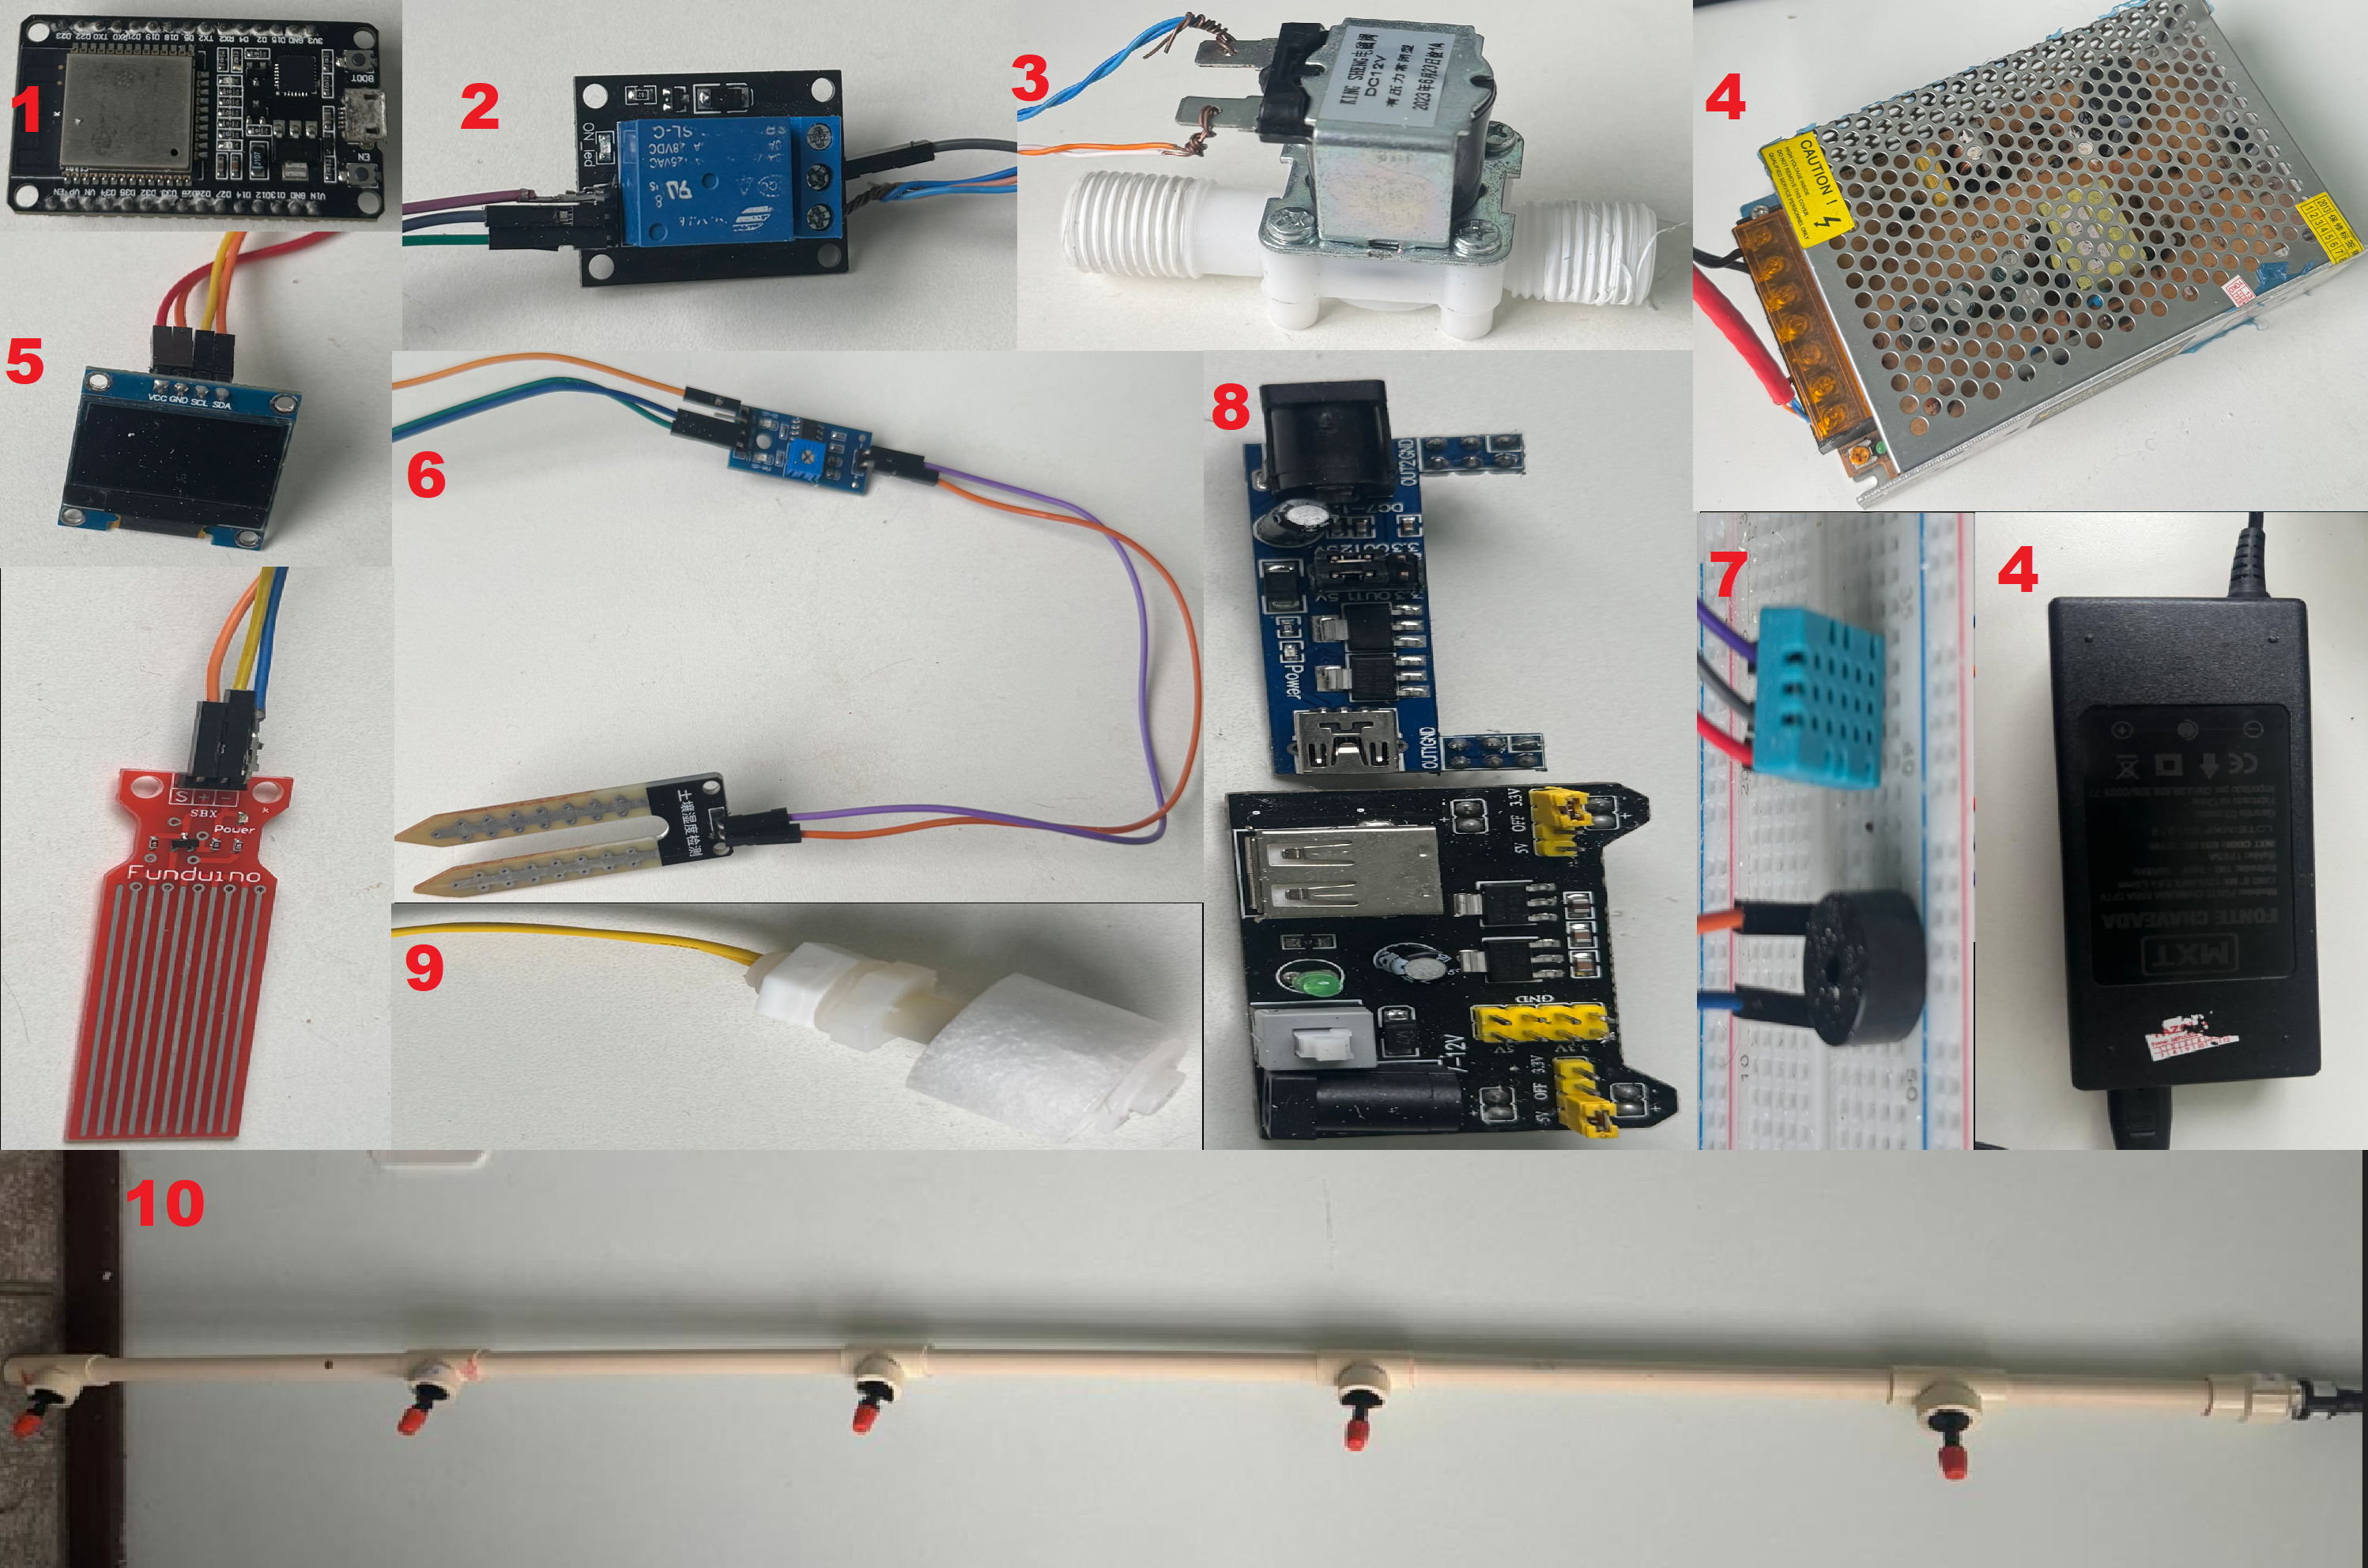
\includegraphics[width=0.8\linewidth]{Figuras/sensores.png}
    \fonte{O Autor (2024)}
    \label{fig:PROTOTIPO}
\end{figure}



\begin{enumerate}[label=\textbf{\arabic*.}]
    \item \textbf{ESP32}: É um microcontrolador dual-core com conectividade Wi-Fi e Bluetooth com SO FreeRTOS.
    \item \textbf{Relé}: O módulo de relé 5V, foi utilizado para controlar a válvula solenoide.
    \item \textbf{Válvula Solenoide}: É um atuador que controla o fluxo de líquidos ou gases. É ativado eletricamente, foi utilizado para ativar o sistema de irrigação.
    \item \textbf{Fonte de Alimentação}: Um componente que converte a corrente alternada (AC) da rede elétrica para corrente contínua (12V DC), fornecendo energia a todos os componentes eletrônicos.
    \item \textbf{Display OLED}: Componente de matriz orgânica de diodos emissores de luz, utilizado para mostrar informações em tempo real ao usuário sobre o sistema de irrigação.
    \item \textbf{Sensor de Umidade do Solo}: Mede a umidade do solo. Foi utilizado no projeto de automação de irrigação para determinar as reais necessidades hídricas das plantas.
    \item \textbf{Sensor de Temperatura e Umidade (DHT11)}: Mede a temperatura e a umidade do ambiente atual, auxiliam nas decisões para o sistema de irrigação.
    \item \textbf{Adaptador de Energia}: É um adaptador de corrente alternada para corrente contínua, utilizado para alimentar dispositivos eletrônicos que necessitam de uma corrente mais baixa de 3 a 5 volts \~.
    \item \textbf{Sistema Hídricos de Irrigação}: Um conjunto de tubos hidráulicos e bicos aspersores utilizado para distribuir água em uma área específica controladamente. 
\end{enumerate}

\subsubsubsection{Plataforma SinricPro}

O Sinric Pro é um serviço de computação em nuvem opensource voltado para dispositivos inteligentes, oferecendo suporte a uma ampla gama de dispositivos que podem ser criados e integrados à plataforma. Uma das principais vantagens da plataforma é a ausência de necessidade de um dispositivo intermediário, como o Echo Dot, Alexa, para integrar e controlar os dispositivos inteligentes. O Sinric Pro realiza essa função diretamente através de seu aplicativo \cref{fig:sinricPro}, eliminando a necessidade de hardware adicional.

O aplicativo do Sinric Pro foi utilizado para permitir o usuário final acompanhar em tempo real a automação de sua horta. Além do aplicativo, foi disponibilizado um dashboard que permite visualizar os dados de até um mês.

\begin{figure}[!h]
    \centering
    \caption{Aplicativo SinricPro}
    \includegraphics[width=1\columnwidth]{Figuras/dashboardsinric.png}
    \fonte{O Autor (2024)}
    \label{fig:sinricPro}
\end{figure}


\section{ANÁLISE DOS DADOS}
Nesta seção, apresentamos e discutimos os resultados obtidos através dos testes realizados tanto em bancada quanto em campo. A análise dos dados é crucial para validar a eficácia do sistema de automação de irrigação proposto, bem como para identificar possíveis melhorias.

\subsection{Testes em Bancada e Laboratório}

Os testes iniciais foram conduzidos em ambiente controlado de laboratório e em ambiente doméstico para assegurar a precisão dos sensores e a confiabilidade do sistema em condições ideais. Foram realizados diversos ensaios para avaliar:

\begin{itemize}
    \item \textbf{Calibração dos Sensores:} Os sensores já vem de fábrica testados, no entanto, é necessário a calibração dos sensores \cref{table:calib1}, garantindo leituras mais precisas e minimizando as variações. 
\end{itemize}
\begin{table}[!htb]
\renewcommand{\tablename}{Quadro}
\captionsetup{justification=raggedright,singlelinecheck=false}
    \caption{Calibração dos Sensores em Laboratório}
    \centering
    \label{table:calib1}
    \begin{tabular}{@{} p{0.2\textwidth} p{0.75\textwidth} @{}}
        \toprule
        \textbf{Sensores} & \textbf{Método de calibração} \\
        \midrule
        Umidade do Solo & Efetuado a coleta de 100 amostragens das leituras do sensor, é posteriormente calculado a média das leituras e aplicado o percentual de umidade do solo. Calibração da voltagem: $ \text{Média\_leituras} \times \frac{3}{2048} $. Calibração em percentual: \text{Porcento} = \text{map}(\text{valor\_analógico}, 4095, 1150, 0, 100). \\
        Sensor de chuva &  Efetuado a coleta de 100 amostragens das leituras do sensor, é posteriormente calculado a média das leituras e aplicado o percentual da leitura da chuva. Calibração da voltagem: $ \text{Média\_leituras} \times \frac{3}{2048} $. Calibração em percentual: \text{Porcento} = \text{map}(\text{valor\_analógico}, 1600, 0, 0, 100). \\
        Sensor Nível D'água &  Apesar de trabalhar apenas com valores de 0 e 1, foi necessário aplicar uma tensão de 0 volts junto a um resistor de 10k para garantir que, quando o sensor estiver aberto, a tensão seja realmente 0. \\
        \bottomrule
    \end{tabular}
    \fonte{O autor (2024)}
\end{table}


\begin{itemize}
    \item \textbf{Precisão dos Sensores:} Comparação entre os dados coletados pelos sensores do sistema e os valores de referência obtidos por instrumentos de medição padrão.
    \item \textbf{Reação do Sistema:} Tempo de resposta do sistema à variação nos dados dos sensores e a execução de comandos de irrigação conforme os parâmetros estabelecidos.
    \item \textbf{Confiabilidade da Comunicação:} Avaliação da estabilidade da comunicação entre os componentes do sistema e o servidor SinricPro.
\end{itemize}

Após todos os testes em laboratório, os resultados mostraram que o sistema responde eficazmente às mudanças nos parâmetros dos sensores, acionando a irrigação quando necessário e interrompendo-a uma vez que os níveis ideais são atingidos.

\subsection{Testes e Aplicação em Campo}

Após a validação em laboratório, o sistema foi implementado em um campo de cultivo real para avaliar seu desempenho em condições ambientais variáveis. Os principais aspectos analisados foram:
\begin{itemize}
    \item \textbf{Calibração dos Sensores em campo:} Por mais que os sensores já estavam calibrados em ambientes de testes em laboratório, foi necessário a calibração dos sensores novamente em campo \cref{table:calib2}, para garantir leituras precisas no ambiente real. 
\end{itemize}
\begin{table}[!htb]
\renewcommand{\tablename}{Quadro}
    \caption{Calibração dos Sensores em Campo}
    \centering
    \label{table:calib2}
    \begin{tabular}{@{} p{0.2\textwidth} p{0.75\textwidth} @{}}
        \toprule
        \textbf{Sensores} & \textbf{Método de calibração} \\
        \midrule
        Umidade do Solo &  Efetuado a coleta de 100 amostragens das leituras do sensor, é posteriormente calculado a média das leituras e aplicado o percentual de umidade do solo. Calibração da voltagem: $ \text{Média\_leituras} \times \frac{3}{2048} $. Calibração em percentual: \text{Porcento} = \text{map}(\text{valor\_analógico}, 4095, 1300, 0, 100). \\
        Sensor de chuva &  Efetuado a coleta de 100 amostragens das leituras do sensor, é posteriormente calculado a média das leituras e aplicado o percentual da leitura da chuva. Calibração da voltagem: $ \text{Média\_leituras} \times \frac{3}{2048} $. Calibração em percentual: \text{Porcento} = \text{map}(\text{valor\_analógico}, 1750, 0, 0, 100). \\
        Sensor Nível D'água &  Apesar de trabalhar apenas com valores de 0 e 1, foi necessário aplicar uma tensão de 0 volts junto a um resistor de 10k para garantir que, quando o sensor estiver aberto, a tensão seja realmente 0. \\
        \bottomrule
    \end{tabular}
    \fonte{O autor (2024)}
\end{table}
\begin{itemize}
    \item \textbf{Eficiência da Irrigação:} Monitoramento da quantidade de água utilizada e comparação com métodos tradicionais de irrigação. Observou-se uma redução significativa no consumo de água, evidenciando a eficiência do sistema.
    \item \textbf{Impacto no Crescimento das Plantas:} Análise do desenvolvimento das plantas irrigadas pelo sistema automatizado comparado com aquelas irrigadas manualmente. As plantas irrigadas automaticamente apresentaram um crescimento mais uniforme e saudável.
    \item \textbf{Feedback do Usuário:} Coleta de dados sobre a usabilidade e satisfação do usuário final, por meio de um questionário e conversas pessoais.
\end{itemize}

    
    Para avaliar a eficácia da automação, foi utilizado um formulário com escala Likert de 5 pontos (1 = Discordo totalmente, 5 = Concordo totalmente). O formulário foi enviado ao usuário final e o \cref{tab:eficacia} apresenta os resultados do questionário de satisfação.
    
\begin{table}[h!]
\centering
\renewcommand{\tablename}{Quadro}
\captionsetup{justification=raggedright,singlelinecheck=false}
\caption{Resultados da avaliação de eficácia da automação}
\label{tab:eficacia}
\begin{tabular}{llccccc}
\hline
\multicolumn{2}{c}{} & \multicolumn{5}{c}{\textbf{Respostas}} \\
\cline{3-7}
\multicolumn{2}{c}{\textbf{Questões}} & \textbf{Concordo Totalmente} & \textbf{Concordo} & \textbf{Indeciso} & \textbf{Discordo} & \textbf{Discordo Totalmente} \\
\hline
Questão 1 & & 1 & 0 & 0 & 0 & 0 \\
Questão 2 & & 0 & 0 & 1 & 0 & 0 \\
Questão 3 & & 1 & 0 & 0 & 0 & 0 \\
Questão 4 & & 1 & 0 & 0 & 0 & 0 \\
Questão 5 & & 1 & 0 & 0 & 0 & 0 \\
Questão 6 & & 1 & 0 & 0 & 0 & 0 \\
Questão 7 & & 1 & 0 & 0 & 0 & 0 \\
Questão 8 & & 0 & 1 & 0 & 0 & 0 \\
Questão 9 & & 1 & 0 & 0 & 0 & 0 \\
\hline
\textbf{Total} & & \textbf{7} & \textbf{1} & \textbf{1} & \textbf{0} & \textbf{0} \\
\hline
\end{tabular}
\fonte{O autor(2024)}
\end{table}



Em suma, os dados obtidos indicam que o sistema de automação de irrigação não só é eficaz na gestão hídrica como também promove um uso mais sustentável dos recursos naturais. A automação também permitiu um gerenciamento mais adequado de tempo, uma vez que a automação permite a configuração de horários específicos para iniciar a irrigação.

\section{CONCLUSÃO}

Ao concluir os estudos verificou-se que o sistema de automação de irrigação desenvolvido atende aos requisitos propostos, demonstrando a sua capacidade de operação tanto em ambientes controlados quanto em campo. O sistema se mostrou eficaz no monitoramento e controle da umidade do solo, ajustando a distribuição de água segundo as necessidades das plantas em tempo real. A integração dos diversos sensores e atuadores permitiu uma resposta rápida e precisa às variações ambientais, garantindo uma utilização eficiente dos recursos hídricos. Além disso, a conectividade Wi-Fi proporcionada pelo ESP32 possibilitou o monitoramento remoto e a coleta de dados, facilitando a análise e o ajuste das estratégias de irrigação.

Os resultados da pesquisa evidenciam que a implementação de sistemas de irrigação automatizados apresentam benefícios significativos, dentre os resultados observados incluem:

\begin{itemize}
    \item \textbf{Redução no Consumo de Água:} O sistema otimiza o uso da água, garantindo que apenas a quantidade necessária seja aplicada, contribuindo para a sustentabilidade ambiental.
    \item \textbf{Melhoria na Qualidade das Culturas:} As plantas irrigadas automatizadamente apresentaram melhor desenvolvimento e produtividade.
    \item \textbf{Facilidade de Uso:} A integração com a plataforma SinricPro facilita o monitoramento e controle do sistema, tornando-o acessível mesmo para usuários com pouca experiência em tecnologia.
\end{itemize}

No entanto, para obter esses resultados, foram enfrentados desafios constantes. O acesso à tecnologia de qualidade e de baixo custo foi uma das principais dificuldades. Até mesmo os hardwares utilizados para o projeto apresentaram-se indisponíveis para aquisição em diversos sites de e-commerce e marketplaces, sendo necessária a importação desses componentes. Esse processo resultou em atrasos significativos no andamento do projeto. Outro ponto crucial foi o desenvolvimento de um firmware robusto, capaz de executar todas as tarefas em tempo real e garantir a confiabilidade do sistema.

É importante salientar que os resultados alcançados são provenientes de apenas um estudo de caso específico. Entre as limitações atuais do projeto, destaca-se a dificuldade de implementação em larga escala e a necessidade de otimização do hardware, bem  como a integração de novos sensores, o armazenamento adequado dos dados, configurações dinâmicas, e a oferta de controles acessíveis aos usuários finais. Esses fatores são essenciais para garantir a eficiência e a escalabilidade do sistema.

Já para as pesquisas futuras que englobem esse mesmo tema, é importante focar na replicabilidade e adaptação do sistema em diferentes tipos de culturas e condições climáticas. Isso visa validar e aprimorar a solução proposta, tornando-a mais robusta e versátil. O sucesso da automação na irrigação depende de uma análise contínua e de melhorias iterativas que incorporem os avanços tecnológicos. Além disso, é crucial atender às necessidades específicas de cada ambiente, garantindo que a solução seja eficiente e adaptável.

Por fim, como sugestões de melhorias para o projeto, destaca-se o tratamento e a estruturação adequada dos dados coletados pelos sensores. A implementação de um servidor centralizado para o processamento desses dados é fundamental para aumentar a eficiência do sistema. Além disso, a escalabilidade do projeto e a oferta de configurações dinâmicas para os usuários finais são aspectos importantes a serem considerados. Garantir a confidencialidade e o controle total dos dados e do sistema automatizado também são prioridades que devem ser tratadas como pontos-chave da expansão do projeto.


\postextual%% Elementos pós-textuais
\newpage
\printbibliography%% Referências

%% Fim do documento
\end{document}
